% =======================
% Chapter: Word Embedding Algorithms
%
% Author: Daniel Wehner
%

% -----------------------------------------------------------------------------------------------------------------------------------------------------
\section{Word Embedding Algorithms}
\label{sec:word_embs}

\vspace*{-2mm}
% -----------------------------------------------------------------------------------------------------------------------------------------------------
% Chapter Introduction
\subsection{Introduction}
\label{sec:word_embs_intro}

Word embeddings form the basis for many sentence embedding algorithms. Therefore, this chapter introduces in more detail what word embeddings are, what approaches exist and how these approaches work. Section \vref{sec:w2v} introduces \textit{word2vec}, while the two subsequent sections are dedicated to \textit{FastText} and \textit{Attract-Repel}, respectively (cf. sections \vref{sec:fasttext} and \vref{sec:attract_repel}). The last section \vref{sec:word_embs_acquisition} finally shows how we acquired word embedding models for later experiments. Available pre-trained vectors were downloaded while others had to be trained from scratch. The section will also provide training details such as which values were used for the hyper-parameters of the respective models.

% -----------------------------------------------------------------------------------------------------------------------------------------------------
% Word2Vec
\subsection{Word2Vec}
\label{sec:w2v}

In order to learn dense word representations, \citep{Mikolov.2013a} introduced a neural approach they called \textit{word2vec}. This algorithm was considered a major breakthrough in the \gls{nlp} community by the time it was published. The learning process of \textit{word2vec} is guided by an \textbf{auxiliary task} which is inspired by language modeling \citep{Bengio.2003}. In contrast to language models which predict the next word in the sequence given all previous words, \textit{word2vec} either predicts the center word given the context words or the context words given the center word. The first variant is called \textit{\gls{cbow}}, while the second one is referred to as \textit{Skip-Gram}. The following paragraphs refer to the \textit{Skip-Gram} architecture, but the concepts are in general transferable to the \textit{\gls{cbow}} variant as well. Figure \vref{fig:skipgram_detail} provides a visual illustration of the explanations:

% Figure: Skip-gram model in detail
\begin{figure}[h]
	\centering
	\begin{tikzpicture}[
		scale=0.335,
		every node/.style={scale=0.7},
		box/.style={rounded corners,dashed}
	]

		%\node[rotate=90] at (-12,0) {\highlight{center word}};
		\node[rotate=90] at (37,0) {\highlight{context words}};

		\draw[box,fill=lightgray!10] (-11,-12) rectangle (-5,14);
		\draw[box,fill=lightgray!10] (-3,-12) rectangle (7,14);
		\draw[box,fill=lightgray!10] (9,-12) rectangle (15,14);

		\node[align=center] at (-8,12) {$\vert \mathcal{V} \vert \times 1$ \\ $\bm{\widehat{v}}_{w_c}$};
		\node[align=center] at (-8,-8) {\highlight{One-hot} \\ \highlight{word vector} \\ \highlight{center word}};

		\node[align=center] at (2,12) {$d \times \vert \mathcal{V} \vert$ \\ $\bm{E}$};
		\node[align=center] at (2,-8) {\highlight{Word embedding matrix}};

		\node[align=center] at (12,12) {$d \times 1$ \\ $\bm{v}_{w_c}$};
		\node[align=center] at (12,-8) {\highlight{Word emb.} \\ \highlight{for center word}};

		\node[align=center] at (19,14) {$\vert \mathcal{V} \vert \times d$ \\ $\bm{U}$};
		\node[align=center] at (25,14) {$\vert \mathcal{V} \vert \times 1$ \\ $\bm{u}_{w_o}^{\intercal} \bm{v}_{w_c}$};
		\node[align=center] at (30,14) {$\vert \mathcal{V} \vert \times 1$ \\ soft-max};
		\node[align=center] at (35,14) {$\vert \mathcal{V} \vert \times 1$ \\ truth};

		\node at (-4,0) {\Large $\times$};
		\node at (8,0) {\Large $=$};

		\node at (-8,0) {$\begin{bmatrix} 0 \\ 0 \\ 0 \\ 0 \\ 0 \\ 1 \\ 0 \\ 0 \\ 0 \end{bmatrix}$};
		\node at (2,0) {$
			\begin{bmatrix*}[r]
				\bullet 	& \hdots 	& 0.2 	& \hdots & \bullet \\[3.2mm]
				\bullet 	& \hdots 	& -1.4 	& \hdots & \bullet \\[3.2mm]
				\bullet 	& \hdots 	& 0.3 	& \hdots & \bullet \\[3.2mm]
				\bullet 	& \hdots 	& -0.1 	& \hdots & \bullet \\[3.2mm]
				\bullet 	& \hdots 	& 0.1 	& \hdots & \bullet \\[3.2mm]
				\bullet 	& \hdots 	& 0.5 	& \hdots & \bullet
			\end{bmatrix*}$};
		\node at (12,0) {$
			\begin{bmatrix*}[r]
				0.2 	\\[3.2mm]
				-1.4	\\[3.2mm]
				0.3 	\\[3.2mm]
				-0.1	\\[3.2mm]
				0.1 	\\[3.2mm]
				0.5
			\end{bmatrix*}$};

			\draw[thick] (16,-3.5) rectangle (22,3.7);
			\draw[thick] (16,-3.5) -- (22,5) -- (22,12.2) -- (16,3.7);
			\draw[thick] (16,3.7) -- (22,-5) -- (22,-12.2) -- (16,-3.5);

		\node at (25,8.75) {$
			\begin{bmatrix*}[r]
				0.2 		\\[3.2mm]
				0.3		\\[3.2mm]
				0.1 		\\[3.2mm]
				\vdots 	\\[3.2mm]
				0.7
			\end{bmatrix*}$};

		\node at (30,8.75) {$
			\begin{bmatrix*}[r]
				0.08 	\\[3.2mm]
				0.10	\\[3.2mm]
				0.05 	\\[3.2mm]
				\vdots 	\\[3.2mm]
				\textcolor{tud9c}{0.65}
			\end{bmatrix*}$};
			\node at (35,8.75) {$\begin{bmatrix} 0 \\[3.2mm] 0 \\[3.2mm] 0 \\[3.2mm] \vdots \\[3.2mm] \textcolor{tud9c}{1} \end{bmatrix}$};
			
		\node at (25,0.1) {$
			\begin{bmatrix*}[r]
				0.7 		\\[3.2mm]
				0.3		\\[3.2mm]
				0.1 		\\[3.2mm]
				\vdots 	\\[3.2mm]
				-0.1
			\end{bmatrix*}$};

		\node at (30,0.1) {$
			\begin{bmatrix*}[r]
				\textcolor{tud9c}{0.65} 	\\[3.2mm]
				0.10	\\[3.2mm]
				0.05 	\\[3.2mm]
				\vdots 	\\[3.2mm]
				0.03
			\end{bmatrix*}$};
			\node at (35,0.1) {$\begin{bmatrix} 0 \\[3.2mm] \textcolor{tud9c}{1} \\[3.2mm] 0 \\[3.2mm] \vdots \\[3.2mm] 0 \end{bmatrix}$};

		\node at (25,-8.75) {$
			\begin{bmatrix*}[r]
				0.5 		\\[3.2mm]
				0.7		\\[3.2mm]
				0.1		\\[3.2mm]
				\vdots 	\\[3.2mm]
				0.4
			\end{bmatrix*}$};

		\node at (30,-8.75) {$
			\begin{bmatrix*}[r]
				\textcolor{tud9c}{0.40} 	\\[3.2mm]
				0.15	\\[3.2mm]
				0.05 	\\[3.2mm]
				\vdots 	\\[3.2mm]
				0.30
			\end{bmatrix*}$};
			\node at (35,-8.75) {$\begin{bmatrix} 0 \\[3.2mm] 0 \\[3.2mm] 0 \\[3.2mm] \vdots \\[3.2mm] \textcolor{tud9c}{1} \end{bmatrix}$};

	\end{tikzpicture}
	\caption[Word2vec's skip-gram model architecture in detail]{The Skip-gram model in detail.
		Image taken and adapted from Manning: \url{https://www.youtube.com/watch?v=ERibwqs9p38}
		(Lecture recording from Stanford university; retrieved: September 04, 2019).}
	\label{fig:skipgram_detail}
\end{figure}

Given the center word $w_c^{(t)}$ at time step $t$, the \textit{Skip-Gram} model has to predict the surrounding words which are given by a sliding window of size $m$ centered on $w_c^{(t)}$. To this end, $w_c^{(t)}$ which is represented as a one-hot vector $\bm{\widehat{v}}_{w_c^{(t)}} \in \mathbb{R}^{\vert \mathcal{V} \vert \times 1}$, is first multiplied by a shared embedding matrix $\bm{E} \in \mathbb{R}^{d \times \vert \mathcal{V} \vert}$, where $d$ is the desired dimensionality of the resulting word embeddings. This matrix contains the weights of the network connecting the input layer to the single hidden layer (with identity activation). The weights in matrix $E$ represent the word embeddings once the model is fully trained. Since the input vector has the one-hot property, the vector-matrix multiplication retrieves one specific column from the matrix, namely the respective (intermediate) embedding of the center word $\bm{v}_{w_c^{(t)}}$.

\textbf{The model must be provided with a supervision signal} in order to adjust the weights during training. In machine learning, this signal is usually obtained by comparing the predictions of the model with the desired output (supervised learning). This results in a training loss whose value is dependent on how far off the model was with its predictions. Based on the loss, the model parameters are adjusted to a greater or lesser extent. However, the training corpus does not have any dedicated labels in this context. Instead, the words in the corpus themselves are used. This approach can be considered a mixture of supervised and unsupervised learning which is commonly known as \textbf{self-supervision}. The labels which are used by \textit{Skip-Gram} are given by the one-hot vectors of the respective context words. To obtain the prediction of the model, one must further multiply the center word embedding by a matrix $\bm{U} \in \mathbb{R}^{\vert \mathcal{V} \vert \times d}$. The resulting vector then serves as input to a soft-max activation which yields a probability distribution over all possible words in the vocabulary $\mathcal{V}$. To be more precise, each word has two representations: One center word representation (contained in matrix $\bm{E}$) and a context word representation (contained in matrix $\bm{U}$). Matrix $\bm{U}$ is needed only for the training procedure and is discarded in the end. During training, the \textit{Skip-Gram} architecture attempts to \textbf{maximize the negative log-probability of the context words given the center word}:

\vspace*{-6mm}
\begin{align}
	\mathcal{J}(\bm{\theta})
		&= -\frac{1}{T} \sum_{t=1}^T \sum_{\substack{-m \le j \le m \\ j \ne 0}}
			\log p(w^{(t+j)} \vert w_c^{(t)}; \bm{\theta}), \\
	\intertext{where the probability is given by the soft-max activation:}
	p(o \vert c)
		&= \frac{\exp\{ \bm{u}_{w_o}^{\intercal} \bm{v}_{w_c}\}}{
			\sum_{\ell=1}^{\vert \mathcal{V} \vert} \exp\{ \bm{u}_{w_\ell}^{\intercal} \bm{v}_{w_c}\}}.
\end{align}
\vspace*{-2mm}

Vector $\bm{\theta}$ denotes the parameters of the model. In this case these are the entries of the matrices $\bm{E}$ and $\bm{U}$. $T$ is the number of words in the training corpus whereas $t$ represents the index into the training corpus. The latter must not be confused with $o$ (context) and $c$ (center) which are indices into the vocabulary $\mathcal{V}$. $\bm{u}_{w_o}^{\intercal} \bm{v}_{w_c}$ is called the scoring function $s(c, o)$.

One property of \textit{word2vec} is that the learned embeddings do not only capture \textbf{syntactical features} of natural language, but incorporate \textbf{semantic aspects} of words as well. \citep{Mikolov.2013c} detected this desirable property by defining nine syntactic and five semantic tasks/questions, e.\,g. \texttt{Adjective-Adverb} (syntactic) or \texttt{Man-Woman} (semantic). The task is to answer questions like \textit{`What is the word that is related to king in the same sense as man is related to woman?'}. The authors were able to demonstrate that such questions can be answered by performing simple algebraic operations on the corresponding word vectors: $\bm{v}_{king} - \bm{v}_{man} + \bm{v}_{woman} \approx \bm{v}_{queen}$ (cf. figure \vref{fig:word2vec_vector_operations}).

\begin{figure}[h]
  	\centering
    	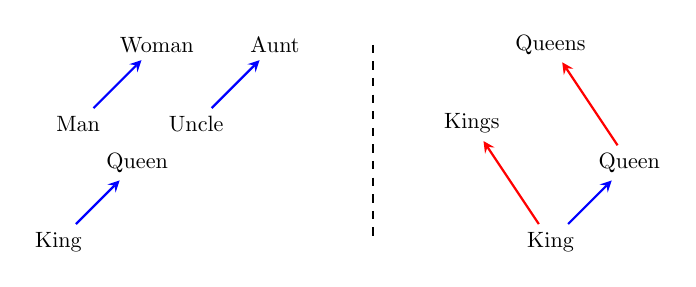
\begin{tikzpicture}[
	scale=0.5,
	every node/.style={scale=0.8},
	arr/.style={-stealth,thick}
]
	
	\node (M) at (0,0) {Man};
	\node (W) at (2,2) {Woman};
	\draw[arr,blue] (M) -- (W);
	
	\node (U) at (3,0) {Uncle};
	\node (A) at (5,2) {Aunt};
	\draw[arr,blue] (U) -- (A);
		
	\node (K1) at (-0.5,-3) {King};
	\node (Q1) at (1.5,-1) {Queen};
	\draw[arr,blue] (K1) -- (Q1);

	\draw[dashed,thick] (7.5,2) -- (7.5,-3);

	\node (K2) at (12,-3) {King};
	\node (Ks) at (10,0) {Kings};
	\node (Q2) at (14,-1) {Queen};
	\node (Qs) at (12,2) {Queens};

	\draw[arr,red] (K2) -- (Ks);
	\draw[arr,red] (Q2) -- (Qs);
	\draw[arr,blue] (K2) -- (Q2);
\end{tikzpicture}
	
  	\caption[Evaluation of word embeddings using similarity tasks]
  	{Similarity tasks can be solved by performing simple algebraic vector operations. The image was taken and adapted from
	\citep{Mikolov.2013c}.}
	\label{fig:word2vec_vector_operations}
\end{figure}

% -----------------------------------------------------------------------------------------------------------------------------------------------------
% FastText
\subsection{FastText}
\label{sec:fasttext}

Despite the great impact \textit{word2vec} had, \citep{Bojanowski.2017} could identify drawbacks. The authors observed that \textbf{the algorithm treats words as atomic units}. This design choice entails problems for words not contained in the training corpus. A large amount of \textbf{\gls{oov} words} is the consequence. It is particularly difficult to learn robust word embeddings for morphologically rich languages like e.\,g. Turkish. In order to address this issue, \citep{Bojanowski.2017} \textbf{enrich the \textit{Skip-Gram} model with sub-word information, where words are considered bags of character $n$-grams}. The word embedding is then defined as the sum of the respective $n$-gram embeddings. Given that the training corpus is sufficiently large, this method basically avoids any \gls{oov} words. If a word did not exist in the training data, its embedding can nevertheless be obtained by summing the respective $n$-gram embeddings. \citep{Bojanowski.2017} were inspired by \citep{Schuetze.1993} and \citep{Wieting.2016a} who introduced similar concepts.

In order to formalize this idea, let $w$ denote an arbitrary word in the vocabulary $\mathcal{V}$. $\mathcal{G}_w$ denotes the set of $n$-grams the word $w$ consists of. A dedicated vector representation $\bm{z}$ is learned for each $n$-gram appearing in the training corpus. \citep{Bojanowski.2017} subsequently replace the original scoring function of \textit{word2vec} by the sum of all character $n$-grams of $w$:

\begin{equation}
	s(c, o) = \sum_{g \in \mathcal{G}_{w_c}} \bm{z}_g^{\intercal} \bm{u}_{w_o}
\end{equation}

The inventors of \textit{FastText} suggest that $n$ be chosen to be in the range from 3 to 6. The authors present an example: Let $n$ be set to 3. The $n$-grams of the word \textit{`where'} are given by: \texttt{<wh}, \texttt{whe}, \texttt{her}, \texttt{ere}, \texttt{re>}. Before the creation of the $n$-grams a word is enclosed in angle brackets (\texttt{<...>}).

% -----------------------------------------------------------------------------------------------------------------------------------------------------
% Attract-Repel
\subsection{Attract-Repel}
\label{sec:attract_repel}

\citep{Mrksic.2017} suggest to incorporate linguistic constraints into the learning process to improve the quality of the word embeddings. Examples for such constraints are \textbf{synonymy/antonymy relationships} between words. Synonymy constraints are introduced to reduce the distance between embeddings representing words with a similar meaning (\textit{attract}) while antonymy relationships allow for pushing vectors further away from each other if the words they represent have contradictory meanings (\textit{repel}). Such relationships can be obtained from lexical resources like e.\,g. \textit{WordNet} \citep{Miller.1995}. In general, two approaches exist how such additional constraints can be incorporated into the process of embedding creation: \ding{182} \textbf{By training word vectors from scratch while respecting the linguistic constraints} or \ding{183} \textbf{by reusing existing word representations which are fine-tuned such that the embeddings obey these constraints}. The authors call this procedure \textbf{semantic specialization}. \textit{Attract-Repel} implements the latter approach and was inspired by techniques called \textit{retro-fitting} \citep{Faruqui.2015}, \textit{Paragram} \citep{Wieting.2015} and \textit{counter-fitting} \citep{Mrksic.2016}.

The inventors of \textit{Attract-Repel} define $S$ and $A$ to be the sets of synonymous and antonymous word pairs, respectively. $(\bm{x}_l, \bm{x}_r)$ describes such a pair, where the words are given by their corresponding vectorial representations. In each training iteration, one mini-batch $\mathcal{B}$ is used consisting of $k_1$ synonymous word pairs ($\mathcal{B}_S$) and $k_2$ antonymous word pairs ($\mathcal{B}_A$). Let further denote $\mathcal{N}_S = \{ (\bm{t}_l^1, \bm{t}_r^1), \dots, (\bm{t}_l^{(k_1)}, \bm{t}_r^{(k_1)}) \}$ the set of negative examples for the synonymous word pairs. A similar set $\mathcal{N}_A = \{ (\bm{t}_l^1, \bm{t}_r^1), \dots, (\bm{t}_l^{(k_2)}, \bm{t}_r^{(k_2)}) \}$ be defined for the antonymous pairs. \\
The negative counterpart of a word pair $(\bm{x}_l, \bm{x}_r)$ is selected from the other words in batch $\mathcal{B}$. For synonymous word pairs, $\bm{t}_l$ is the nearest neighbor of $\bm{x}_l$, while $\bm{t}_r$ is the nearest neighbor of $\bm{x}_r$. Similarly, for antonymous word pairs, $\bm{t}_l$ is selected to be the vector with the largest distance to $\bm{x}_l$, while $\bm{t}_r$ is the vector with the largest distance to $\bm{x}_r$. The cost function of the model is given by:

\begin{align}
	\label{eq:cost_syn}
	\mathcal{J}(\mathcal{B}_S)
		&=\sum_{(\bm{x}_l, \bm{x}_r) \in \mathcal{B}_S}
			\big(\tau(\delta_{syn} + \bm{x}_l^{\intercal} \bm{t}_l - \bm{x}_l^{\intercal} \bm{x}_r) +
			\tau(\delta_{syn} + \bm{x}_r^{\intercal} \bm{t}_r - \bm{x}_l^{\intercal} \bm{x}_r)\big) \\
	\label{eq:cost_ant}
	\mathcal{J}(\mathcal{B}_A) 
		&=\sum_{(\bm{x}_l, \bm{x}_r) \in \mathcal{B}_A}
			\big(\tau(\delta_{ant} + \bm{x}_l^{\intercal} \bm{x}_r - \bm{x}_l^{\intercal} \bm{t}_l) +
			\tau(\delta_{ant} + \bm{x}_l^{\intercal} \bm{x}_r - \bm{x}_r^{\intercal} \bm{t}_r)\big) \\
	\mathcal{J}(\mathcal{B})
		&= \mathcal{J}(\mathcal{B}_S) + \mathcal{J}(\mathcal{B}_A) + \text{regularization term}
\end{align}

$\tau(x)$ denotes the \textbf{hinge loss} and $\delta_{syn}$ is a hyper-parameter specifying how much closer the synonymous words should be in contrast to the negative examples ($\delta_{ant}$ is defined analogously for antonymous word pairs). For intuition, consider equation \vref{eq:cost_syn} which shows the part of the cost function concerning synonymous constraints. If $\bm{x}_l$ and $\bm{x}_r$ are nearby vectors, their dot product will be large. This is desirable, since the two words are synonymous. Subtracting this quantity reduces the cost. At the same time, a large dot product of $\bm{x}_l$ with its negative example $\bm{t}_l$ is punished by adding the respective term. In their experiments the authors minimize the objective function using the \textbf{AdaGrad} optimization technique \citep{Duchi.2011}. Training for five epochs without early stopping was found to be sufficient to obtain sensibly fine-tuned word representations. The authors could produce significant quality improvements for low-resource languages and observed enhanced performance in downstream tasks.

% -----------------------------------------------------------------------------------------------------------------------------------------------------
% Acquisition of Word Embeddings
\subsection{Acquisition of Word Embeddings}
\label{sec:word_embs_acquisition}

The word embeddings presented in this chapter play an important role, since they form the basis for sentence embedding algorithms which will be covered in  chapter \vref{sec:sent_embs}. Table \vref{tab:word_embs_acquisition} summarizes how these word embeddings were obtained:

% Table: Overview word embeddings
\vspace*{2mm}
\begin{table}[h]
	\centering
	\renewcommand{\arraystretch}{2.2}
	\scalebox{1.0}{
	\begin{tabularx}{0.95\textwidth}{| c | X | c | c | c | c | c | c | c | c | c |}
		\hline
		\cellcolor{tud9c!50}							 								&
		\cellcolor{tud9c!50}															&
		\multicolumn{5}{c |}{\cellcolor{tud9c!50}\textbf{Embedding source}}	 			&
		\cellcolor{tud9c!50}								 							&
		\multicolumn{3}{c |}{\cellcolor{tud9c!50}\textbf{Training details}}				\\
		\cellcolor{tud9c!50}\multirow{-2}{*}{\textbf{Nr.}}								&
		\cellcolor{tud9c!50}\multirow{-2}{*}{\textbf{Embedding}}						&
		\cellcolor{tud9c!30}\textbf{EN} 												&
		\cellcolor{tud9c!30}\textbf{DE} 												&
		\cellcolor{tud9c!30}\textbf{RU} 												&
		\cellcolor{tud9c!30}\textbf{TR} 												&
		\cellcolor{tud9c!30}\textbf{KA} 												&
		\cellcolor{tud9c!50}\multirow{-2}{*}{\textbf{Download}}							&
		\cellcolor{tud9c!30}\textbf{Dimen.}			 									&
		\cellcolor{tud9c!30}\textbf{Window size} 										&
		\cellcolor{tud9c!30}\textbf{Architecture}										\\
		\hline\hline

		% word2vec
		\ding{182} 																	&
		\textit{word2vec} 															&
		\faDownload 																	&
		\faDownload																	&
		\faCogs 																		&
		\faCogs																		&
		\faCogs																		&
		\href{https://code.google.com/archive/p/word2vec/}{\linkstyle{Link1}},
		\href{https://deepset.ai/german-word-embeddings}{\linkstyle{Link2}}				&
		300																			&
		10 																			&
		CBOW 
																					\\
		% fastText
		\ding{183} 																	&
		\textit{FastText}																&
		\faDownload 																	&
		\faDownload 																	&
		\faDownload 																	&
		\faDownload 																	&
		\faDownload																	&
		\href{https://fasttext.cc/docs/en/crawl-vectors.html}{\linkstyle{Link}}				&
		300																			&
		- 																			&
		- 
																					\\
		% attract-repel
		\ding{184} 																	&
		\textit{Attract-Repel}															&
		\faDownload 																	&
		\faDownload 																	&
		\faDownload 																	&
		\faDownload 																	&
		\faDownload																	&
		\href{https://drive.google.com/drive/folders/0B_pyA_IW4g-jZHlWWVBfaWRYY0E}
			{\linkstyle{Link}}															&
		300																			&
		- 																			&
		- 																			\\
		\hline
	\end{tabularx}}
	\caption[Sources of word embeddings]{Overview of word embedding acquisition.
		The \faDownload\ symbol indicates that the model was downloaded, whereas the \faCogs\ symbol refers to
		a trained model.}
	\label{tab:word_embs_acquisition}
\end{table}
\vspace*{2mm}
 
\highlight{Availability of pre-trained word embeddings.} Pre-trained embedding spaces for \textit{FastText} and \textit{Attract-Repel} are already publicly available for all target languages. These word vectors were thus downloaded from the respective sources (indicated by the \faDownload\ symbol in table \vref{tab:word_embs_acquisition}). We found \textit{word2vec} vectors for English and German, but unfortunately not for Georgian. This is why we trained these embeddings from scratch (indicated by the \faCogs\ symbol in table \vref{tab:word_embs_acquisition}). For Turkish, only 200-dimensional vectors were available. Different embedding dimensionalities render the results less comparable as already pointed out by \citep{Eger.2019}. Therefore, we chose to train Turkish embeddings as well. Although trained vector representations exist for Russian, we decided to proceed analogously, in order to have similar conditions among the low-resource languages.

\highlight{Training details.} We trained all \textit{word2vec} embeddings on Wikipedia dumps for the respective languages (Russian, Turkish and Georgian). The dumps are provided by Wikimedia\footnote{\url{https://dumps.wikimedia.org/} (retrieved: September 20, 2019)} in an \gls{xml} format. In order to get hold of the plain text which is needed for training, these \gls{xml} files have to be parsed. A module for the Python programming language called  \texttt{WikiExtractor}\footnote{\url{https://github.com/attardi/wikiextractor} (retrieved: September 20, 2019)} was used for this purpose. Table \vref{tab:wikipedia_stats} shows the sizes of the Wikipedia dumps as measured by the number of sentences.

Mikolov and colleagues provide the official C-implementation of \textit{word2vec} on GitHub\github.\footnote{\url{https://github.com/tmikolov/word2vec} (retrieved: September 20, 2019)} For training, we did not change the default hyper-parameters of the script. The training setting is as follows: First of all, the \textit{\gls{cbow}} architecture was used and the window size was set to $m = 10$. We chose a dimensionality of the resulting vectors of $d = 300$. The training process took about 2 hours per language on a \gls{gpu} computer, where the reduced amount of training time is due to smaller data sets as can be seen in table \vref{tab:wikipedia_stats}.

\begin{table}[h]
	\centering
    	\renewcommand{\arraystretch}{1.2}
\scalebox{1.05}{
\begin{tabular}{| c | r | c |}
	\hline
	\rowcolor{tud9c!50}
	\textbf{Language}	&
	\textbf{\# sentences} & 
	\textbf{Version} \\
	\hline\hline
	\textbf{English} 		& 	97,285,870 	&	20.02.2019 	\\
	\textbf{German} 		& 	40,729,339	&	20.09.2018	\\
	\textbf{Russian} 		& 	25,324,234 	&	01.02.2019	\\
	\textbf{Turkish} 		& 	3,797,955	&	01.01.2019	\\
	\textbf{Georgian} 	& 	1,047,780	&	20.07.2016	\\
	\hline
\end{tabular}}
  	\caption[Wikipedia statistics for each language]
		{Number of sentences contained in the Wikipedia dumps for each language. As can be seen, among the languages
 		considered Georgian is by far the one with the fewest resources.}
	\label{tab:wikipedia_stats}
\end{table}

% -----------------------------------------------------------------------------------------------------------------------------------------------------
% Chapter Summary
\subsection{Summary}
\label{sec:word_embs_summary}

In this chapter the concept of word embeddings was introduced. Since most machine learning algorithms are not designed for natural language input, researchers began to devise techniques to obtain vectorial representations of language which are called language embeddings. Mikolov and colleagues introduced a seminal approach they called \textit{word2vec}. It can be trained efficiently on large corpora and captures not only syntactic but also semantic aspects of words. The fact that simple algebraic operations on these vectors suffice to answer similarity questions popularized this algorithm in the \gls{nlp} community.

To account for some drawbacks of the \textit{word2vec} algorithm, other techniques and extensions were proposed. \textit{FastText} extends the \textit{Skip-Gram} model to character $n$-grams which enables it to cope with \gls{oov}-words in a more graceful fashion. \textit{Attract-Repel} explicitly includes linguistic constraints based on synonymy and antonymy relationships to fine-tune existing word embeddings. The idea behind this approach is that synonymous words should be mapped close to each other in the embedding space while antonymous words should be as far apart as possible.

Finally, an overview provided information about where and how the word embeddings were obtained. Pre-trained models for \textit{FastText} and \textit{Attract-Repel} embeddings were available for all target languages and were therefore downloaded from the official websites. Suitable \textit{word2vec} vectors were available only for English and German. For the low-resource languages Russian, Turkish and Georgian they were trained from scratch using the official implementation provided by Mikolov and colleagues.